\section{Recurrent Neural Networks (RNNs)}

\subsection{Hopfield Networks}

\subsubsection{A Two-Dimensional Network}

\begin{figure}[!h]
    \centering
    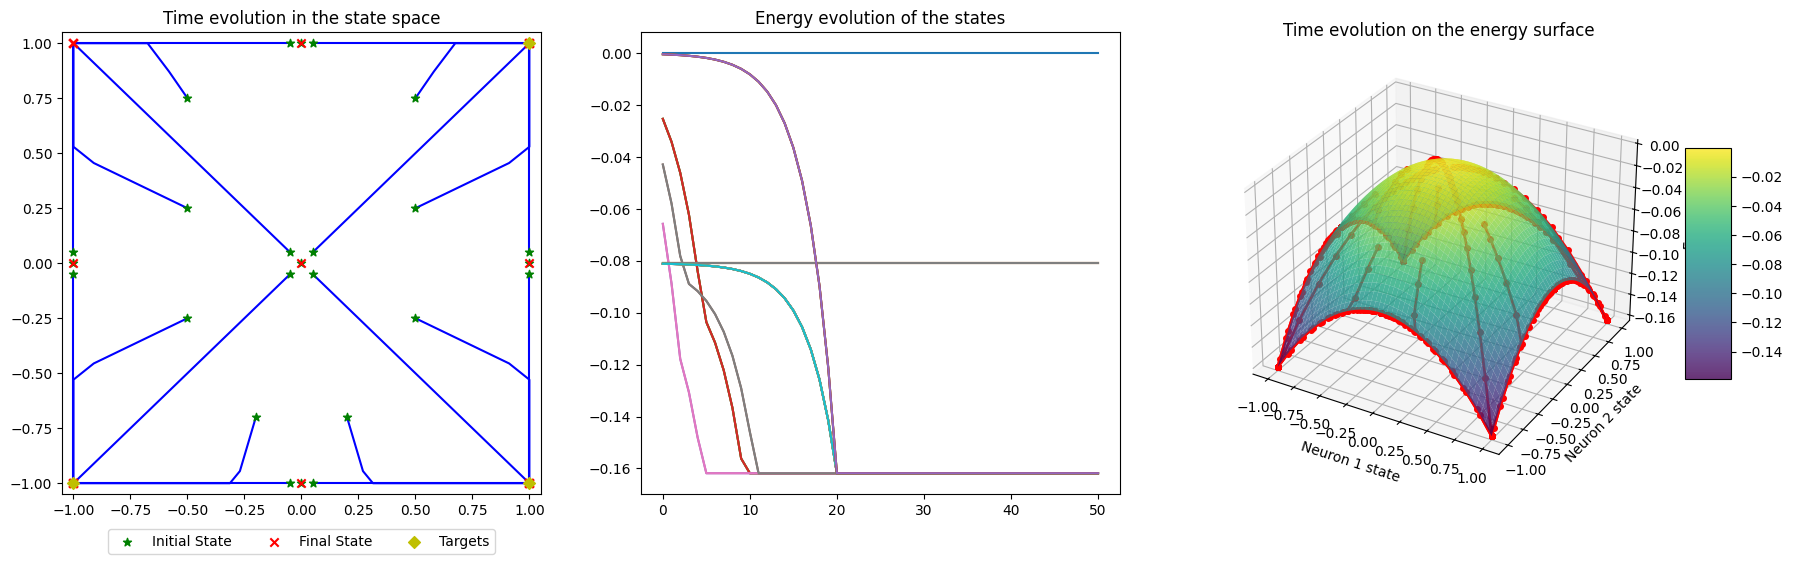
\includegraphics[width=\textwidth]{figures/hopfield-2d-iterations-50.png}
    \caption{Evolution of 2D Hopfield Network over 50 iterations}
    \label{fig:hopfield-2d-iterations-50}
\end{figure}

\paragraph{Spurious Attractors}

The set of targets $S$ used to create the network are all attractors: \verb|[[-1. -1.] [ 1. -1.] [ 1.  1.]]|.
In addition, there are spurious attractors
due to symmetric minima (\verb|[[-1. 1.]]|, Equations \ref{eq:symmetric-attractors-update-rule}, \ref{eq:symmetric-attractors-update-rule-example}),
maxima (\verb|[[ 0. 0.]]|) or saddle points (\verb|[[1. 0.], [ 0. 1.], ...]|) on the energy surface.
That is, symmetry gives rise to attractors also in points symmetric to  or equidistant from the set of targets $S$.

\begin{equation}
    W = \sum_{\bm{s} \in S}{\bm{s}\bm{s}^T} = \begin{bmatrix}
        1 \\ 1
    \end{bmatrix} \begin{bmatrix}
        1 \\ 1
    \end{bmatrix}^T + \begin{bmatrix}
        -1 \\ -1
    \end{bmatrix} \begin{bmatrix}
        -1 \\ -1
    \end{bmatrix}^T + \begin{bmatrix}
        1 \\ -1
    \end{bmatrix} \begin{bmatrix}
        1 \\ -1
    \end{bmatrix}^T = \begin{bmatrix}
        3 & 1 \\
        1 & 3
    \end{bmatrix}
    , \quad
    \min_{\bm{s}} -\frac{1}{2}\bm{s}^T W \bm{s}
\end{equation}

\begin{equation}
    \bm{x}^{(n+1)} = \alpha(W \bm{x}^{(n)})
    , \qquad
    \alpha \big(W \cdot (-\bm{x}^{(n)}) \big) = \alpha (- W \bm{x}^{(n)}) = - \alpha(W \bm{x}^{(n)}) = - \bm{x}^{(n+1)}
    \label{eq:symmetric-attractors-update-rule}
\end{equation}

\begin{equation}
    \alpha \bigg( W \alpha \Big( W \begin{bmatrix}
        0.5 \\ -0.75
    \end{bmatrix} \Big) \bigg) = \begin{bmatrix}
        1 \\ -1
    \end{bmatrix} \in S
    , \qquad
    \alpha \bigg( W \alpha \Big( W \begin{bmatrix}
        -0.5 \\ 0.75
    \end{bmatrix} \Big) \bigg) = \begin{bmatrix}
        -1 \\ 1
    \end{bmatrix} \notin S
    \label{eq:symmetric-attractors-update-rule-example}
\end{equation}

\paragraph{Convergence}

In this network, it may take up to $\approx 20$ iterations to reach an attractor.

\paragraph{Stability}

An unstable attractor is one such that if a pattern is initialised in an unstable attractor, it remains there.
But just a small perturbation of the initial state would cause it to converge to a stable attractor instead.

Minima minimise energy, i.e. are stable (incl. spurious attractors arising due to symmetry).
Maxima or saddle points do not minimise energy, i.e. are unstable.

\paragraph{Design}

To accurately store patterns or memories,
a good associative memory network should \textit{ideally} have
no spurious, nor unstable, attractors.

\pagebreak

\subsubsection{A Three-Dimensional Network}

\begin{figure}[h!]
    \begin{minipage}[t]{0.44\textwidth}
        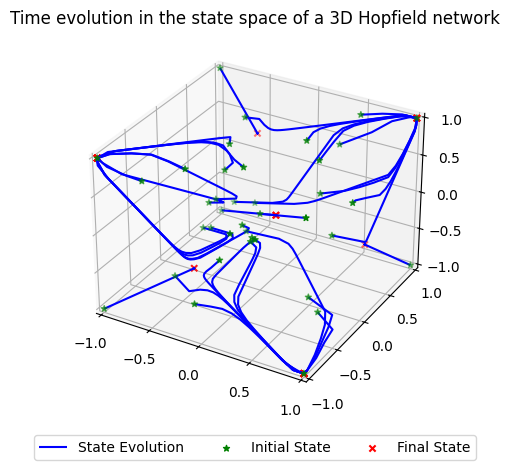
\includegraphics[width=\textwidth]{figures/hopfield-3d-iterations-50-state-space.png}
        \label{fig:hopfield-3d-iterations-50-state-space}
    \end{minipage}
    \begin{minipage}[t]{0.54\textwidth}
        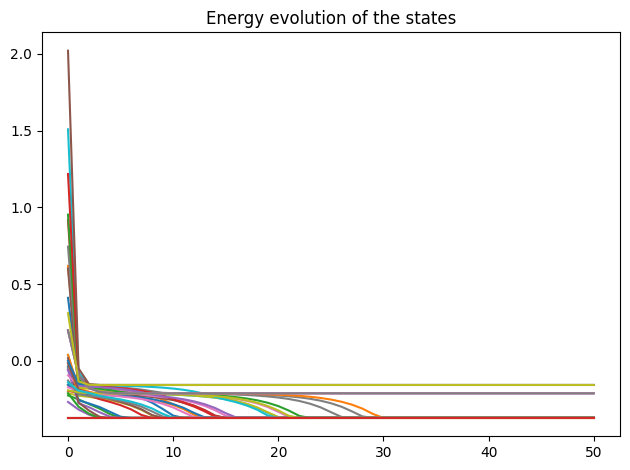
\includegraphics[width=\textwidth]{figures/hopfield-3d-iterations-50-energy-evolution.png}
        \label{fig:hopfield-3d-iterations-50-energy-evolution}
    \end{minipage}
    \caption{Evolution of 3D Hopfield Network over 50 iterations}
\end{figure}

\paragraph{Spurious Attractors}

The set of targets $S$ used to create the network are all attractors:
\verb|[[-1. -1.  1.] [ 1. -1. -1.] [ 1.  1.  1.]]|.
In addition, there are spurious attractors.
These are the midpoints on the edges between the targets:
\verb|[[-0.06 -1. -0.06]| \verb|[-0.06 0.06 1.] [ 1. 0.06 -0.06]]|
\big($\begin{pmatrix}
    \frac{-1 + 1}{2}, & \frac{-1 - 1}{2}, & \frac{1 - 1}{2}
\end{pmatrix} = \begin{pmatrix}
    0, & -1, & 0
\end{pmatrix}$, etc.\big).
And the circumcentre of the triangle formed by the targets:
\verb|[[ 0.367 -0.367  0.367]]|.

\paragraph{Convergence} Like in two dimensions, in most cases it takes $< \approx 20$ iterations to reach an attractor,
but may take up to $30$ or $40$ iterations in a three-dimensional network.

\paragraph{Stability}

\begin{figure}[h!]
    \begin{minipage}[t]{0.44\textwidth}
        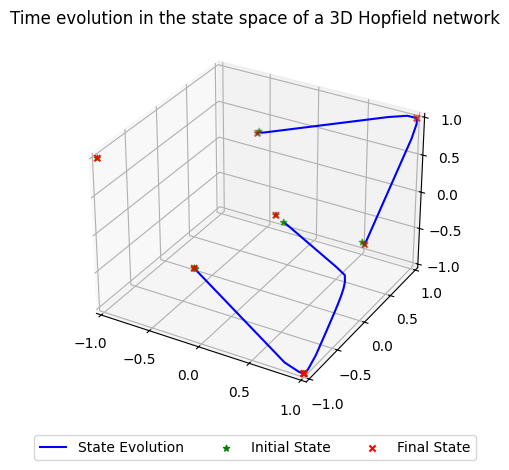
\includegraphics[width=\textwidth]{figures/hopfield-3d-iterations-50-state-space-perturbations.png}
        \label{fig:hopfield-3d-iterations-50-state-space-perturbations}
    \end{minipage}
    \begin{minipage}[t]{0.54\textwidth}
        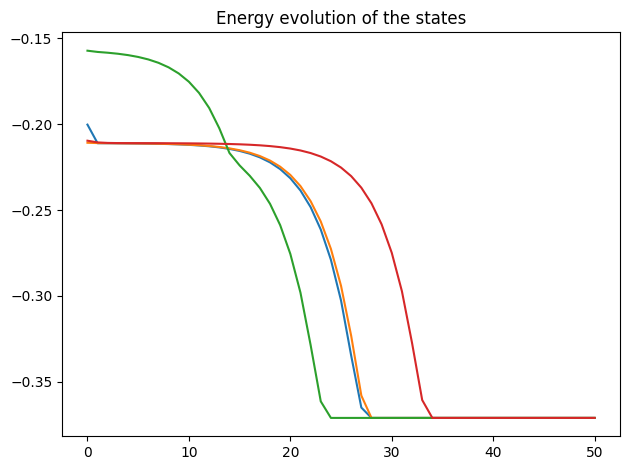
\includegraphics[width=\textwidth]{figures/hopfield-3d-iterations-50-energy-evolution-perturbations.png}
        \label{fig:hopfield-3d-iterations-50-energy-evolution-perturbations}
    \end{minipage}
    \caption{Evolution of 3D Hopfield Network over 50 iterations near spurious attractors}
\end{figure}

Initial points near spurious attractors do not converge to the spurious attractors,
i.e. spurious states may be unstable. An analytical solution could confirm this.

\subsubsection{Digit Recognition with a Higher-Dimensional Network}

A higher-dimensional Hopfield Network can be used to store handwritten digits.
Retrieval from the network can be tested by having it reconstruct digits corrupted by noise.

\paragraph{Reconstruction Capacity}

The Hopfield Network performs very well - better than the untrained human eye -
but is \textit{not always able to reconstruct the noisy digits}.
This is because the additive noise changes the image.
That is, with noise the image's initial state will be farther away from the intended attractor.
If there is too much noise it does not look like the original digit anymore
and may even become more similar (closer) to a different digit (attractor).
In such a case the network produces an incorrect reconstruction.

For noise levels of 0\%, 10\%, 20\%, 30\% and even 40\% the network is always able to reconstruct all digits correctly in the experiments.
From 50\% noise the network begins to make mistakes.
In particular, it makes mistakes between digits with similar patterns, like threes, fives and nines.
It also mistakes an eight for a one, likely because the eight is very narrow in the dataset, which with noise could look like and converge to a one.

\paragraph{Number of Iterations}

\textit{The more noise} there is the farther away from their intended attractors the noisy digits will be
and \textit{the more iterations it takes} for the network to (fully) reconstruct the given digits (i.e. converge to the attractors).

For noise levels of 0\%, 10\%, 20\%, 30\% the network is able to denoise all the correct digits after just one iteration so that the human eye can recognise them.
For full reconstruction (convergence to the attractors) it takes up to $\approx 5, 10, 20$ iterations respectively in the experiments, however.
With 40\% noise after just one iteration it is not possible to decipher anything yet, although after 25 iterations the correct attractors are reached.

\begin{figure}[h!]
    \begin{minipage}[t]{0.24\textwidth}
        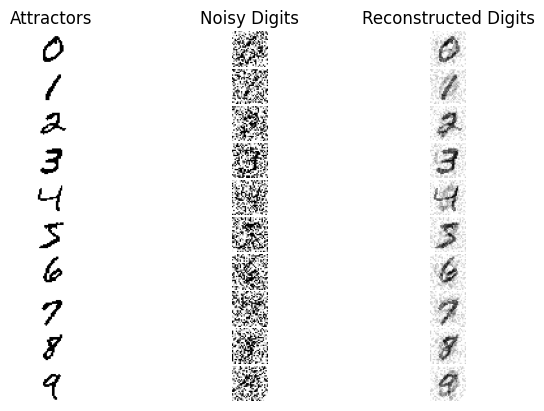
\includegraphics[width=\textwidth]{figures/hopfield-digits-20-noise-1-it.png}
        \label{fig:hopfield-digits-20-noise-1-it}
    \end{minipage}
    \begin{minipage}[t]{0.24\textwidth}
        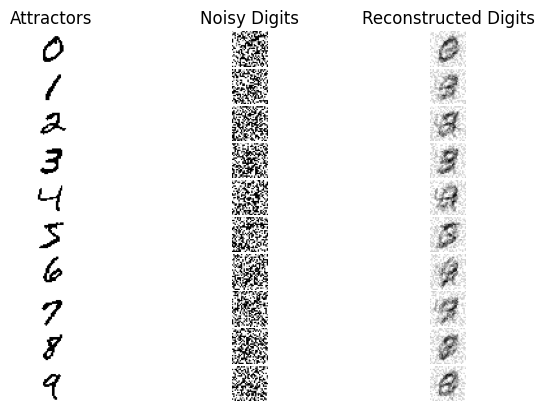
\includegraphics[width=\textwidth]{figures/hopfield-digits-40-noise-1-it.png}
        \label{fig:hopfield-digits-40-noise-1-it}
    \end{minipage}
    \begin{minipage}[t]{0.24\textwidth}
        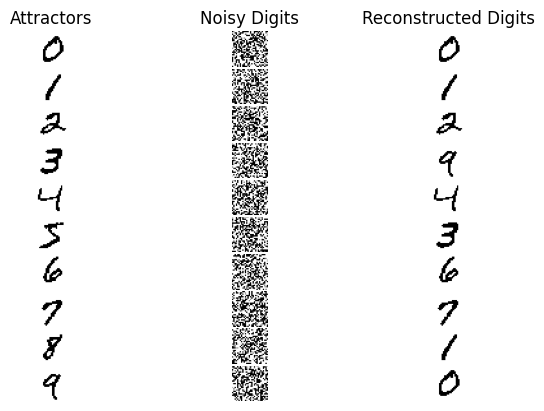
\includegraphics[width=\textwidth]{figures/hopfield-digits-40-noise-25-it.png}
        \label{fig:hopfield-digits-40-noise-25-it}
    \end{minipage}
    \begin{minipage}[t]{0.24\textwidth}
        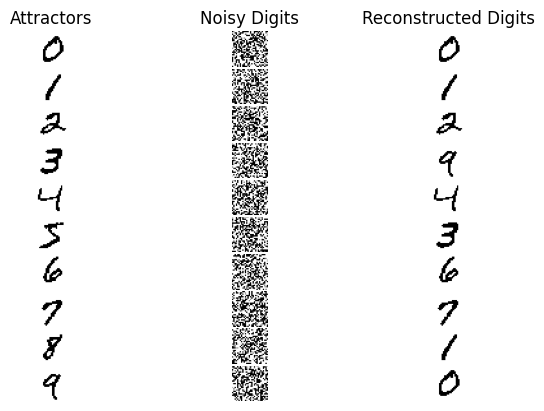
\includegraphics[width=\textwidth]{figures/hopfield-digits-50-noise-50-it.png}
        \label{fig:hopfield-digits-50-noise-50-it}
    \end{minipage}
    \caption{Digit reconstruction: (a) 20\% noise/1 it., (b) 40\%/1, (c) 40\%/25, (d) 50\%/50}
\end{figure}
\vspace{-10pt}

\subsection{Time Series Prediction}

A dynamical system evolves over time, often following physical rules.
The Santa Fe laser data, with 1000 training and 100 test steps, behaves nonlinearly due to e.g. delay, noise.

\subsubsection{Multi-Layer Perceptron (MLP) with One Hidden Layer}

Two hyperparameters are systematically tuned for a single-hidden-layer MLP:
the number of input lags and the size of the hidden layer.
For each setting, the model is trained using K-fold (time series) cross-validation\footnote{
    Cross-validation is a validation technique that makes better use of limited amounts of available training data,
    at the expense of being more computationally and time-intensive.
    If there are temporal (or spatial, etc.) correlations as in time series cross-validation,
    care has to be taken when splitting the data to respect chronological order and prevent data leakage.
} and its out-of-sample performance is recorded.
The training regime (optimiser, etc.) is fixed for a fair and simple comparison,
exploring the influence of both input history and network capacity on time series prediction accuracy.

The MLP performs poorly with smaller lag values.
Increasing the lag to 50 or 100 and the number of hidden units to 50 improves the performance
and the model is able to better recognise the drop that occurs and after which the time series is reset.

Lag 100 \& 50 hidden units give the best performance (MSE 2462.667) on the test set.

\subsubsection{Long-Short-Term Memory (LSTM)}

Recurrent neural networks (RNNs) are neural architectures with loops that allow information to persist across time steps.
Long Short-Term Memory (LSTM) networks are a type of RNN designed to better learn \textit{long-term} dependencies, which standard RNNs struggle with due to the vanishing gradient problem.
LSTMs achieve this by maintaining a memory cell and using gating mechanisms to regulate how much - controlled by sigmoid activations $\in [0, 1]$ - at each time step information is input, forgotten, or output.
Variants include LSTMs with peephole connections and Gated Recurrent Units (GRUs), the latter of which combines the input and forget gates into a single update gate. \citep{olah2015understanding}

Increasing the lag for the LSTM also improves its performance, although the LSTM also performs well already with a smaller lag value.
It is especially able to better recognise the unexpected drop / change in the series, also with a 10 times smaller lag.
It is important to also tune the number of hidden units.
100 hidden units are sufficient to model the time series; such a model performs better than a model with the same lag but more or fewer (e.g. 50 or 200) hidden units.

Lag 50 \& 100 hidden units give the best performance (MSE 418.086) on the test set.
Lag 10 \& 100 hidden units give second-best performance (MSE 1643.964) on the test set.
Further experiments might reveal an even better configuration, e.g. $10 \leq$ lag $\leq 50$.

\subsubsection{Model Evaluation}

The MLP requires a much larger number of inputs (i.e. lag) in order to be able to learn the underlying trend in the time series,
and even so performs worse especially when it comes to predicting unexpected events.
The LSTM requires fewer inputs due to its more sophisticated architecture, and is better able to predict unexpected events.
The LSTM clearly outperforms in terms of performance and in terms of its requirements for past data availability in order to be able to make predictions.

\begin{figure}[h!]
    \begin{minipage}[t]{0.48\textwidth}
        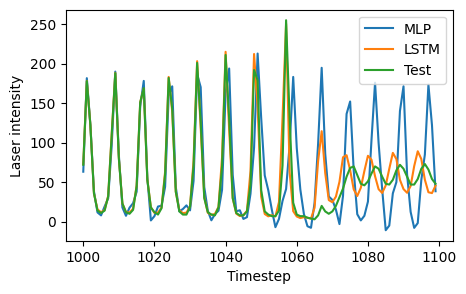
\includegraphics[width=\textwidth]{figures/time-series-santa-fe-results-mlp-lstm.png}
    \end{minipage}
    \hfill
    \begin{minipage}[t]{0.48\textwidth}
        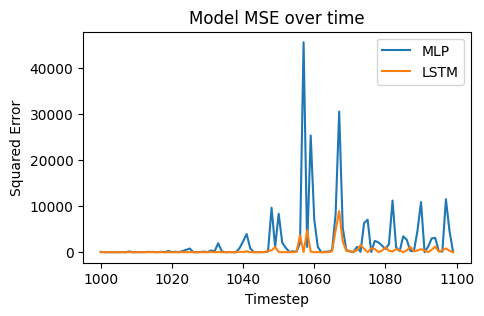
\includegraphics[width=\textwidth]{figures/time-series-santa-fe-errors-mlp-lstm.png}
    \end{minipage}
    \caption{Predictions on test set (MLP MSE: $2462.667$, LSTM MSE: $418.086$)}
    \label{fig:time-series-santa-fe-results-mlp-lstm}
\end{figure}
